% Emerald Publishing - Construction Innovation Submission Template
% by Oleksandr Melnyk
% Ver 0.0.4
% Based on: https://www.emeraldgrouppublishing.com/journal/ci#author-guidelines


\documentclass{article}

\usepackage[english]{babel}

% Set page size and margins
% Replace `letterpaper' with `a4paper' for UK/EU standard size
\usepackage[a4paper,top=2cm,bottom=2cm,left=3cm,right=3cm,marginparwidth=1.75cm]{geometry}

% Useful packages
\usepackage{amssymb}
\usepackage{siunitx}
\PassOptionsToPackage{hyphens}{url}\usepackage{hyperref}
\usepackage[utf8]{inputenc}
\usepackage[right]{lineno}
\usepackage{csquotes}
\usepackage{booktabs}
\usepackage{longtable}
\usepackage{adjustbox}
\usepackage{array}
\usepackage{url}
\usepackage{titlesec}
\usepackage{amsmath}
\usepackage{cleveref}
\usepackage{graphicx}
\usepackage{subcaption}
%\usepackage[compatibility=false]{caption}
\usepackage{authblk}
\usepackage{xcolor} % Load the xcolor package for color options
\renewcommand{\thetable}{\Roman{table}}
\usepackage{float}
\usepackage{caption}

% Define a new format for \subsection
\titleformat{\subsection}
  {\mdseries\itshape\large} % Medium series, italic shape, and large font size
  {\thesubsection}{1em}{} % Numbering, spacing, and the section title itself

\titleformat{\subsubsection}
  {\mdseries\itshape\large}  % Same formatting as for \subsection
  {\thesubsubsection}{1em}{} % Numbering, spacing, and the section title itself

% Emerald Harvard Citation Style

\usepackage[english]{babel}
\usepackage[style=authoryear,backend=biber,natbib=true,maxcitenames=2,uniquelist=false]{biblatex}
\addbibresource{Bibliography.bib} % your .bib file

% Customizing biblatex for Harvard style
% Customizing biblatex for Harvard style
\DeclareNameAlias{sortname}{family-given}
\DeclareNameAlias{default}{family-given}

\renewbibmacro{in:}{}
\DeclareFieldFormat[article]{title}{\mkbibquote{#1}\addcomma}
\DeclareFieldFormat[book]{title}{\mkbibemph{#1}\addcomma}
\DeclareFieldFormat[bookinbook]{title}{\mkbibemph{#1}\addcomma}
\DeclareFieldFormat[inbook]{title}{\mkbibquote{#1}\addcomma}
\DeclareFieldFormat[incollection]{title}{\mkbibquote{#1}\addcomma}
\DeclareFieldFormat[inproceedings]{title}{\mkbibquote{#1}\addcomma}
\DeclareFieldFormat[manual]{title}{\mkbibemph{#1}\addcomma}
\DeclareFieldFormat[misc]{title}{\mkbibemph{#1}\addcomma}
\DeclareFieldFormat[thesis]{title}{\mkbibemph{#1}\addcomma}
\DeclareFieldFormat[unpublished]{title}{\mkbibquote{#1}\addcomma}
\DeclareFieldFormat[patent]{title}{\mkbibemph{#1}\addcomma}
\DeclareFieldFormat[report]{title}{\mkbibemph{#1}\addcomma}
\DeclareFieldFormat[online]{title}{\mkbibquote{#1}\addcomma}
\DeclareFieldFormat[software]{title}{\mkbibemph{#1}\addcomma}
\DeclareFieldFormat[booklet]{title}{\mkbibemph{#1}\addcomma}
\DeclareFieldFormat[periodical]{title}{\mkbibemph{#1}\addcomma}
\DeclareFieldFormat[standard]{title}{\mkbibemph{#1}\addcomma}

\DeclareFieldFormat[article]{journaltitle}{\iffieldundef{shortjournal}{\mkbibemph{#1}\addcomma}{\mkbibemph{\printfield{shortjournal}}\addcomma}}
\DeclareFieldFormat{volume}{\bibstring{volume}~#1}
\DeclareFieldFormat{number}{\bibstring{number}~#1}

% Definitions for "Vol." and "No."
\DefineBibliographyStrings{english}{
  volume = {Vol.},
  number = {No.}
}

\renewbibmacro*{volume+number+eid}{%
  \printfield{volume}%
  \setunit*{\addspace}%
  \printfield{number}%
  \setunit{\addcomma\space}%
  \printfield{eid}}

\renewbibmacro*{journal+issuetitle}{%
  \usebibmacro{journal}%
  \setunit*{\addcomma\space}%
  \usebibmacro{volume+number+eid}%
  \setunit{\addcomma\space}%
  \usebibmacro{issue+date}}

\renewbibmacro*{publisher+location+date}{%
  \printlist{publisher}%
  \iflistundef{location}
    {\setunit*{\addcomma\space}}
    {\setunit*{\addcolon\space}}%
  \printlist{location}%
  \setunit*{\addcomma\space}%
  \usebibmacro{date}}

\renewcommand*{\bibpagespunct}{\addcomma\space}

% Customizing page field format to prevent duplication
% \DeclareFieldFormat{pages}{%
%   \mkfirstpage[{\mkpageprefix[page]{#1}}]{#1}}

% Customizing citations for Harvard style
\DeclareCiteCommand{\cite}[\mkbibparens]
  {\usebibmacro{prenote}}
  {\usebibmacro{citeindex}%
   \usebibmacro{cite}}
  {\multicitedelim}
  {\usebibmacro{postnote}}

\renewbibmacro*{cite:labelyear+extrayear}{%
  \iffieldundef{labelyear}
    {}
    {\printtext[bibhyperref]{%
       \printfield{labelyear}%
       \printfield{extrayear}}}}

\renewbibmacro*{cite:labeldate+extradate}{%
  \iffieldundef{labelyear}
    {}
    {\printtext[bibhyperref]{%
       \printfield{labelyear}%
       \printfield{extradate}}}}

\AtEveryBibitem{
  \clearfield{month}
  \clearfield{day}
  \ifentrytype{book}{
    \clearlist{location}
  }{}
}

% Formatting "et al." in italics followed by a comma
\DefineBibliographyStrings{english}{
  andothers = {\textit{et al.},}
}

\DeclareFieldFormat[article]{volume}{\bibstring{jourvol}\addnbspace #1}
\DeclareFieldFormat[article]{number}{\bibstring{number}\addnbspace #1}
\DeclareFieldFormat[article]{volume}{Vol. #1}
\DeclareFieldFormat[article]{number}{No. #1}
% Customizing DOI field format to lowercase "doi"
%\DeclareFieldFormat{doi}{\bibstring{doi}\addcolon\space\url{#1}}

% Customizing URL field format to "available at:"
\DeclareFieldFormat{url}{\bibstring{available at}\addcolon\space\url{#1}}
\DeclareFieldFormat{urldate}{\mkbibparens{accessed \addspace#1}}

% Customizing urldate to match the required format
\DeclareFieldFormat{urldate}{%
  \mkbibparens{accessed\space%
    \thefield{urlday}\addspace%
    \mkbibmonth{\thefield{urlmonth}}\addspace%
    \thefield{urlyear}}}


% Configure cleveref
\crefformat{figure}{#2Figure~#1#3}
\Crefformat{figure}{#2Figure~#1#3}
\crefformat{table}{#2Table~#1#3}
\Crefformat{table}{#2Table~#1#3}
\crefformat{section}{#2Section~#1#3}
\Crefformat{section}{#2Section~#1#3}

%Front Matter

\author[1]{Benjamin Vadurel}
\author[1]{Emilien Komlenovic}

\affil[1]{Université Claude Bernard Lyon 1}

\title{Terrorism Dataset analysis}

\begin{document}
\maketitle


%%%%%%%%% ABSTRACT
\begin{abstract}
   This study performs data mining techniques on the University of Maryland's comprehensive terrorism database covering events from 1970 to 2021. We employ multiple analytical approaches, including tetrachoric correlation analysis, clustering algorithms, and temporal pattern recognition, to uncover underlying relationships between terrorist events and their geopolitical context. Our methodology encompasses preprocessing categorical data through one-hot encoding and applying various clustering techniques (K-Means, Agglomerative Clustering, K-Modes, and DBSCAN) to identify distinct attack patterns. We obtained preliminary results, such as data correlations, and established links with the events in the real-world.

%add 6 keywords
\textbf{Keywords:} correlation; pattern recognition; cluster analysis; temporal anomaly detection
\end{abstract}
%\linenumbers
%%%%%%%%% BODY TEXT
\section{Introduction}

The dataset describes each terrorist event that occurred from 1970 to 2021, it gives data about the date, the place and the individuals involved in the event. The dataset \cite{GTD} is made by the University of Maryland and the data come from various organizations : 
\begin{itemize}
    \item The Pinkerton Global Intelligence Service (PGIS) : a private security agency.
    \item Center for Terrorism and Intelligence Studies (CETIS) :  a research center dedicated to the study of terrorist groups, political and religious extremism, and various types of covert intelligence operations.
    \item Institute for the Study of Violent Group (ISVG) : a research center focused on insurgency, terrorism, and transnational organized crime.
\end{itemize}


\section{Data Description}

\subsection{Fields and content}

Each row of the dataset aim to describe a terrorist event with 135 columns. Using the information contained in these columns we can get :
\begin{itemize}
    \item The date the event occurred
    \item The place the event occurred
    \item Some descriptors for the attack (has the attack succeeded, has the attacker killed itself, etc..)
    \item The attack type representing the method used (ex : Assassination, Bombing, etc..)
    \item 3 Inclusion criteria : \\
    \textit{crit1} means that the attacks was made for political, economic, religious or social goal instead of personal motive (like profit). \\
    \textit{crit2} concerns the attacks that were made to coerce, intimidate or publicize large audiences. \\
    \textit{crit3} represent if the attacks respect the international humanitarian law.
    \item The weapon used during the attack
    \item The target of the attack
    \item The name of the terrorist group
    \item If the attack was claimed
    \item The material and human damages the attack caused
\end{itemize}

A complete documentation for the data can be found in the 
\href{https://github.com/ekomlenovic/SecurityDataset/blob/main/data/Codebook.pdf}{\textit{Codebook}}.

\subsection{Preprocessing}
The dataset was originally encoded for human understanding and sharing but unfit for data analysis. For the categorical data, each field are duplicated having the category label and the associated category in text. For those, we decided to remove the duplicated fields and one-hot encode the categories.
In the dataset, unknown data are usually represented by -9, we replaced those by NaN.

\subsection{Visualization}

As we are working with spatial data, we can visualize it by building a map representing the attacks such as Figure \ref{fig:terrorism-map} where each red dot represent an attack. Most of the attacks are located on populated areas of the world.

\begin{figure}[!htb]
    \centering
    \includegraphics[width=1\linewidth]{img//Description/terrorism_map.png}
    \caption{Map displaying each positions where a terrorist event happened from 1970 to 2021}
    \label{fig:terrorism-map}
\end{figure}

\section{Problems}

Our goal is to correlate data on terrorist attacks with the corresponding geopolitical context. To achieve this, we have established several sub-questions:
\begin{itemize}
    \item Match population data by year for each country
    \item Find attacks that can be associated together
    \item Identify frequent patterns in the data: Uncovering recurring trends or associations to better understand the underlying dynamics.
    \item Detect anomalies in the data: Highlight irregularities that may indicate geopolitical problems.
    \item Analyze temporal relationships: Studying the evolution of events over time.
\end{itemize}

\section{Data processing}

\subsection{Variable correlations}

To process the correlation among the variables, we'll use the tetracoric correlation which is efficient in our case because the dataset contains a lot of boolean variables.

\begin{figure}[htbp]
    \centering
    \[
        v = a \cdot \frac{d}{\frac{b}{c}}
    \]

    \vspace{1em}
    \centering
    $a, b, c, d$  Corresponding to the factor of the 2 variables in the confusion matrix 
\end{figure}

$$
    corr = \cos\left(\frac{\pi}{1+\sqrt{v}}\right)
$$
Using this coefficient, we produce the heatmap given in Figure \ref{fig:tetracoric_heatmap} and using it we can make several observations.

We can first focus on the inclusion criterion : we observe that for each criterion we find a correlation with military targeting. The criterion 3 indicating that the attacks doesn't follow the international humanitarian laws is often correlated with targets like educational institution, citizen, properties, businesses and religious figures. Moreover, criterion 3 attack seems to have a correlation with the claiming method such as letters.

Hijacking attacks are often correlated to targets such as maritime ports and airports which is coherent to the nature of the attack.

Finally, abortion-related attacks are correlated to attack on infrastructure which is also coherent as abortion-related attacks often happen in abortion clinics as specified in the \href{https://github.com/ekomlenovic/SecurityDataset/blob/main/data/Codebook.pdf}{\textit{Codebook}}

\subsection{Clustering}

The objective here is to highlight the presence of groups in the attacks. As we're dealing with a large dataset, we'll split the dataset based on the time periods.

All the clustering we built, were based on the \textit{attack\_type}, \textit{the target\_type}, \textit{the claim mode} and some additional descriptors. Using these fields, we first performed clustering using 4 different algorithms : K-Means\cite{WikipediaKMeans}, Agglomerative Clustering\cite{WikipediaHierarchicalClustering} and K-Modes\cite{Huang1998}. Implementing the automatic k-selection, we evaluated the silhouette score for each cluster size represented in Table \ref{tab:styled_table}. 

\begin{table}[!htb]
    \centering
    \setlength{\tabcolsep}{12pt} % Adjust column spacing
    \renewcommand{\arraystretch}{1.5} % Adjust row spacing
    \begin{tabular}{>{\centering\bfseries}p{2cm}cccc}
        \toprule

        Cluster number & Agglomerative clustering & K-Means & K-Modes \\
        \midrule
        2        & 0.187756        & 0.262278        & 0.197518       \\
        3         & 	0.194116        & 0.21552        & 0.206285     \\
        4         & 0.215864        & 0.187088	       & 0.20739     \\
        5         & 0.192268        & 0.218445        & 0.197518     \\
        6         & 0.209013       & 0.21552        & 	0.197518     \\
        \bottomrule
    \end{tabular}
    \caption{Computed silhouette\cite{WikipediaSilhouette} score for each algorithm depending on the number of cluster}
    \label{tab:styled_table}
\end{table}


We observe in Table \ref{tab:styled_table} that for the 3 methods, silhouette score nears 0,20. As the cluster size does not seems to impacts the quality of the cluster, we will choose arbitrarily 3 clusters. As we're working with spatial data, we can ensure spatial continuity with the agglomerative clustering using a connectivity matrix.

We also tried DBScan algorithm for the clustering, it gives a clustering with 387 clusters and a silhouette score of 0.881. Even if we get a decent silhouette score for this clustering, it's hard to determine a meaning for these clusters.

Figure \ref{fig:clustering-comparison} represents the obtained clustering for the attacks between 2000 and 2010.

\begin{figure}[htbp]
    \centering
    % Première ligne
    \begin{subfigure}{0.45\linewidth}
        \centering
        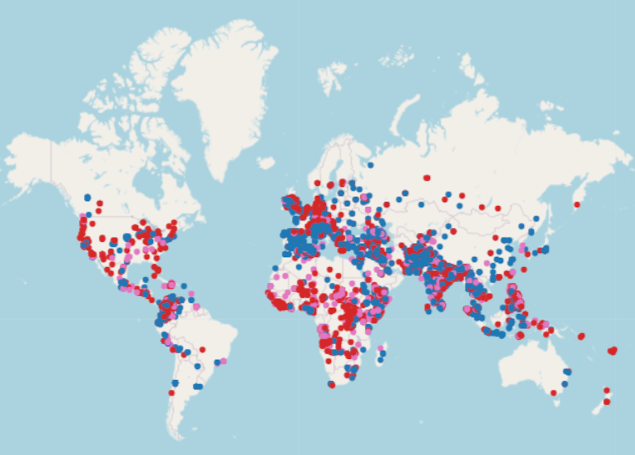
\includegraphics[width=\linewidth]{img//Clustering/Clusters K Means_resized.png}
        \caption{K-Means Clustering (with n\_clusters=3)}
        \label{fig:kmeans}
    \end{subfigure}
    \hfill
    \begin{subfigure}{0.45\linewidth}
        \centering
        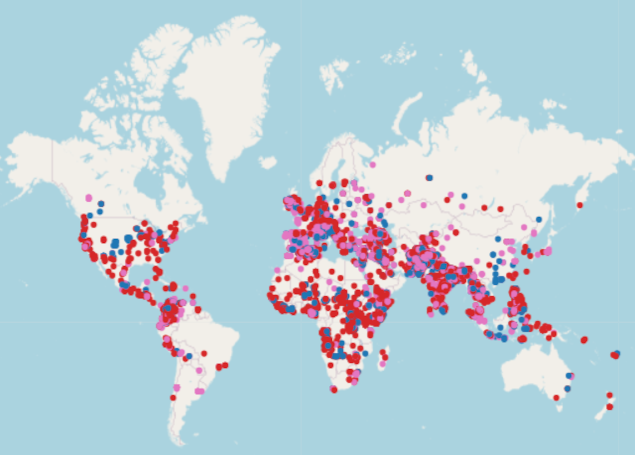
\includegraphics[width=\linewidth]{img//Clustering/Clusters K Mode_resized.png}
        \caption{K-Modes Clustering (with n\_clusters=3)}
        \label{fig:kmodes}
    \end{subfigure}
    
    % Deuxième ligne
    \begin{subfigure}{0.45\linewidth}
        \centering
        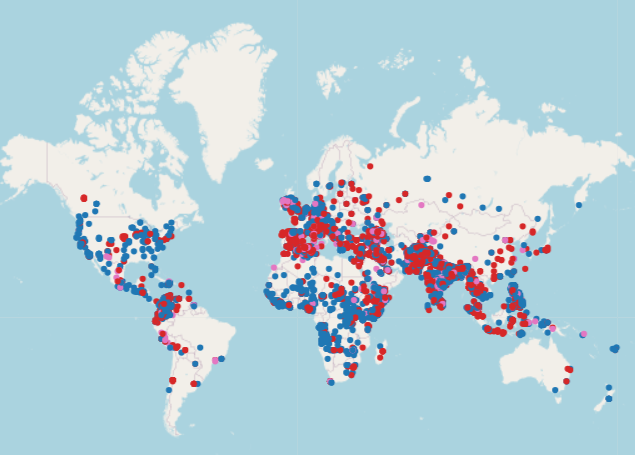
\includegraphics[width=\linewidth]{img//Clustering/Clusters Agglo.png}
        \caption{Agglom. Clustering (with n\_clusters=3)}
        \label{fig:agglo}
    \end{subfigure}
    \hfill
    \begin{subfigure}{0.45\linewidth}
        \centering
        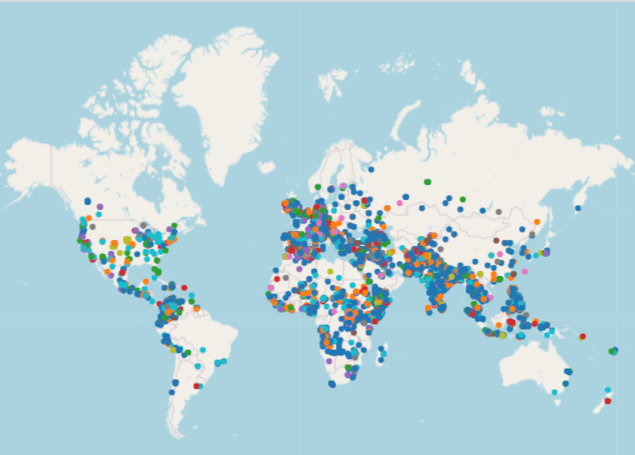
\includegraphics[width=\linewidth]{img//Clustering/Clusters DB Scan_resized.png}
        \caption{DBScan Clustering (with eps=0.5)}
        \label{fig:dbscan}
    \end{subfigure}
    
    \caption{Comparison of Clustering Methods}
    \label{fig:clustering-comparison}
\end{figure}

To better understand the produced clusters, we can observe the plots \ref{fig:kmeans-attributes}, \ref{fig:kmodes-attributes}, \ref{fig:agglo-attributes} representing the proportion of each features present in the clusters. The plot is build from the results obtains by the algorithms with 3 clusters.

The k-modes algorithms has its first cluster containing bombing attacks, the second armed assaults on the police or military and the third contains armed assaults on citizens or properties.

The k-means algorithms has its first cluster containing every attacks targeting citizens such as armed assaults or kidnapping, the second cluster contains bombing attacks on citizen and the third contains bombing on the police which also includes suicide attacks.

The agglomerative clustering has its first cluster containing all kinds of attacks on citizens (assassination, kidnapping and armed assaults), the second mainly contains bombing attacks on citizens and properties and the third contains attacks on the police.

The 3 algorithms produced clustering separating attacks on citizen from the attacks on institutions (such as police and military) and bombing type attack from armed attack or kidnapping.

We won't perform this analysis on the clustering produced by DBScan algorithm as it produced a high number of cluster.


\subsection{Frequent Patterns}

Initially, we search for frequent patterns on the boolean data in the dataset.
Our primary objective was to discover association rules by applying the Apriori algorithm\cite{mlxtend}. However, we observed that no significant frequent patterns emerged.

After preprocessing the dataset, the results changed significantly. The preprocessing allowed us to reveal strong association rules that were not apparent in the raw data.


The criteria \textit{crit1}, \textit{crit2}, and \textit{doubtterr} play a central role in defining armed incidents against military targets. Successful incidents involving firearms have a very high probability of involving military targets. The very strong relationships (high lift, high conviction) suggest that these patterns are significant in the context of terrorism, as illustrated in Figure \ref{fig:fp_lift}.

We aimed to identify patterns between terrorist groups and attack types. However, based on the metrics, we found that there is no consistent pattern.

\subsection{Temporal Analysis}

\subsubsection{Anomaly Detection}

To detect temporal anomalies, we counted the number of attacks per year by country. However, we encountered an issue related to scaling, as countries like Afghanistan and Iraq report a significantly higher number of attacks in certain years, which creates challenges with the scaling of the data.

To address this issue, we computed the deviations from the average for each countries and then visualized the results in \textit{heatmap} Figure \ref{fig:anomaly_detect_heatmap}. The heatmap included in this report represents data for a subset of 50 countries. For the complete version, you can refer to the \href{https://github.com/ekomlenovic/SecurityDataset/blob/main/data_processing/analyses/anomaly_detect_heatmap_full.png}{repository on GitHub}.
We can try to make some analysis based on our results.\\
The years 2010 to 2020 in Afghanistan were marked by the intensification of the Taliban insurgency, the rise of other extremist groups such as ISIS-K, and a series of political and military events that contributed to the resurgence of terrorist attacks in the country.\cite{WikipediaAfghanistan}

Between 1983 and 1997, Colombia was engulfed in a multifaceted conflict involving leftist guerrillas, right-wing paramilitary groups, and drug cartels. Violence, drug trafficking, and political instability made this period ripe for increased terrorist acts.\cite{WikipediaColombia}

From 1977 to 1986, France experienced a pivotal shift in governmental policy, particularly with the election of François Mitterrand, which may have contributed to the rise in violence during this period.\cite{WikipediaMitterrand}

\subsubsection{France over years}

To examine the evolution of the number of attacks in France Figure \ref{fig:ratio_fr} in relation to its population\cite{WorldBankPopulation}, we observed that while the total number of attacks remained relatively stable, the population has significantly increased over time. Consequently, the ratio of attacks per capita has markedly decreased.

\begin{figure}[!htb]
    \centering
    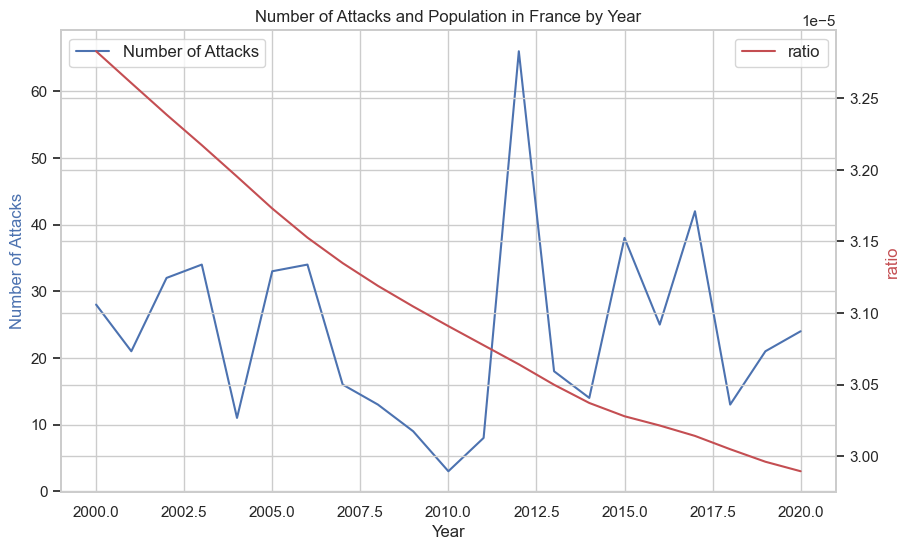
\includegraphics[width=0.5\linewidth]{img/ratio_fr.png}
    \caption{Number of attacks and ratio in France between 2000-2020}
    \label{fig:ratio_fr}
\end{figure}


By highlighting the anomalies in Figure \ref{fig:anomaly-fr} in the number of attacks each months, we can reveal terrorism crisis in France.

As mentioned before, the period from 1978 to 1986 represents the pivotal shift in the governmental politic. During the period going from 1990 to 1997 a lot of attacked were made by the Armed Islamic Group of Algeria more precisely between 1994 and 1996. The attacks in 2011 and 2012 mainly comes from the Corsica region because of political issues.

\begin{figure}[!htb]
    \centering
    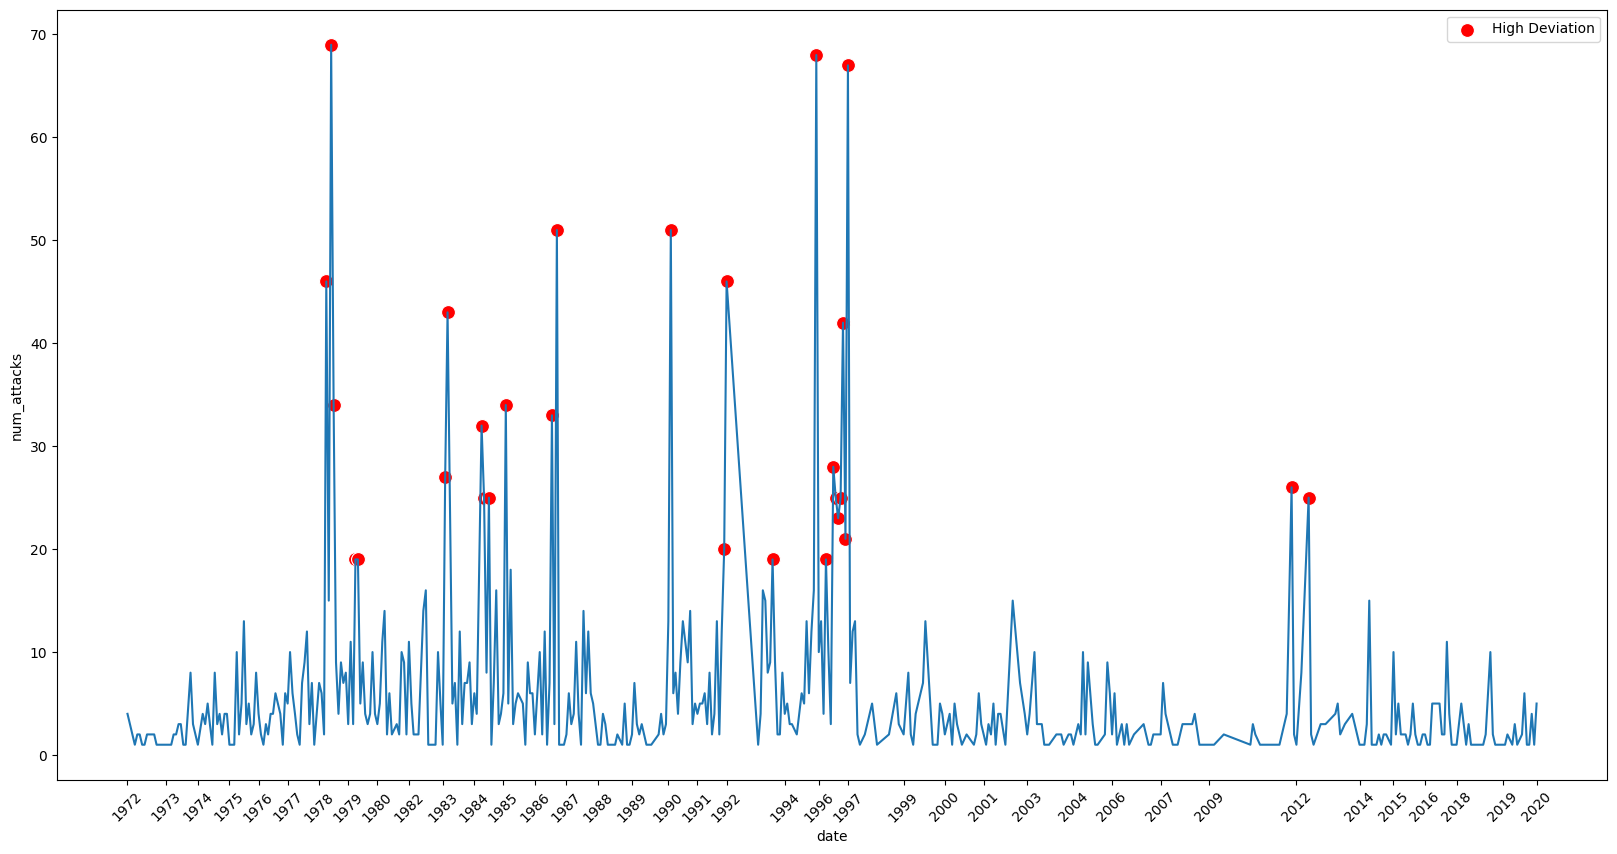
\includegraphics[width=0.75\linewidth]{img//Anomaly/france_anomaly.png}
    \caption{Evolution of the number of attack in France from 1972 to 2020}
    \label{fig:anomaly-fr}
\end{figure}


\newpage
\section{Contributions}

We both worked on data description and the problem statement, as well as data processing. Benjamin focused on variable correlation and clustering, while Emilien worked on frequent pattern analysis and temporal analysis.

\section{Annexe}



\begin{figure}[!htb]
    \centering
    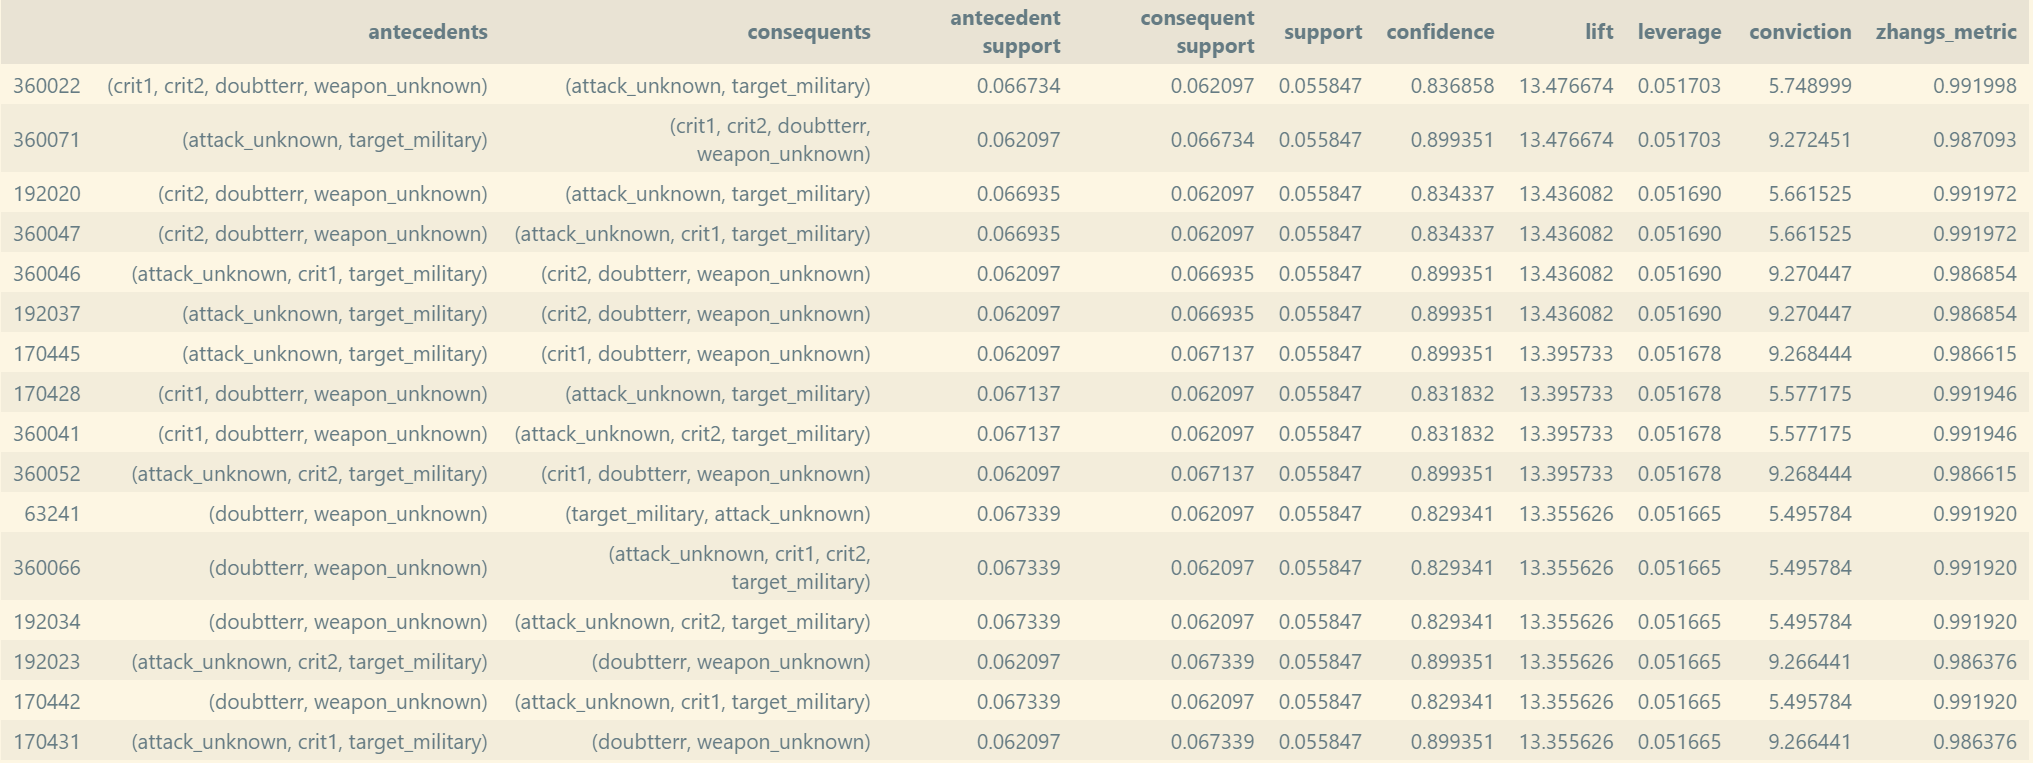
\includegraphics[width=0.8\linewidth]{img/FrequentPattern/fp_lift_1.png}
    \caption{Frequent Pattern Ordered by lift}
    \label{fig:fp_lift}
\end{figure}
\begin{figure}
    \centering
    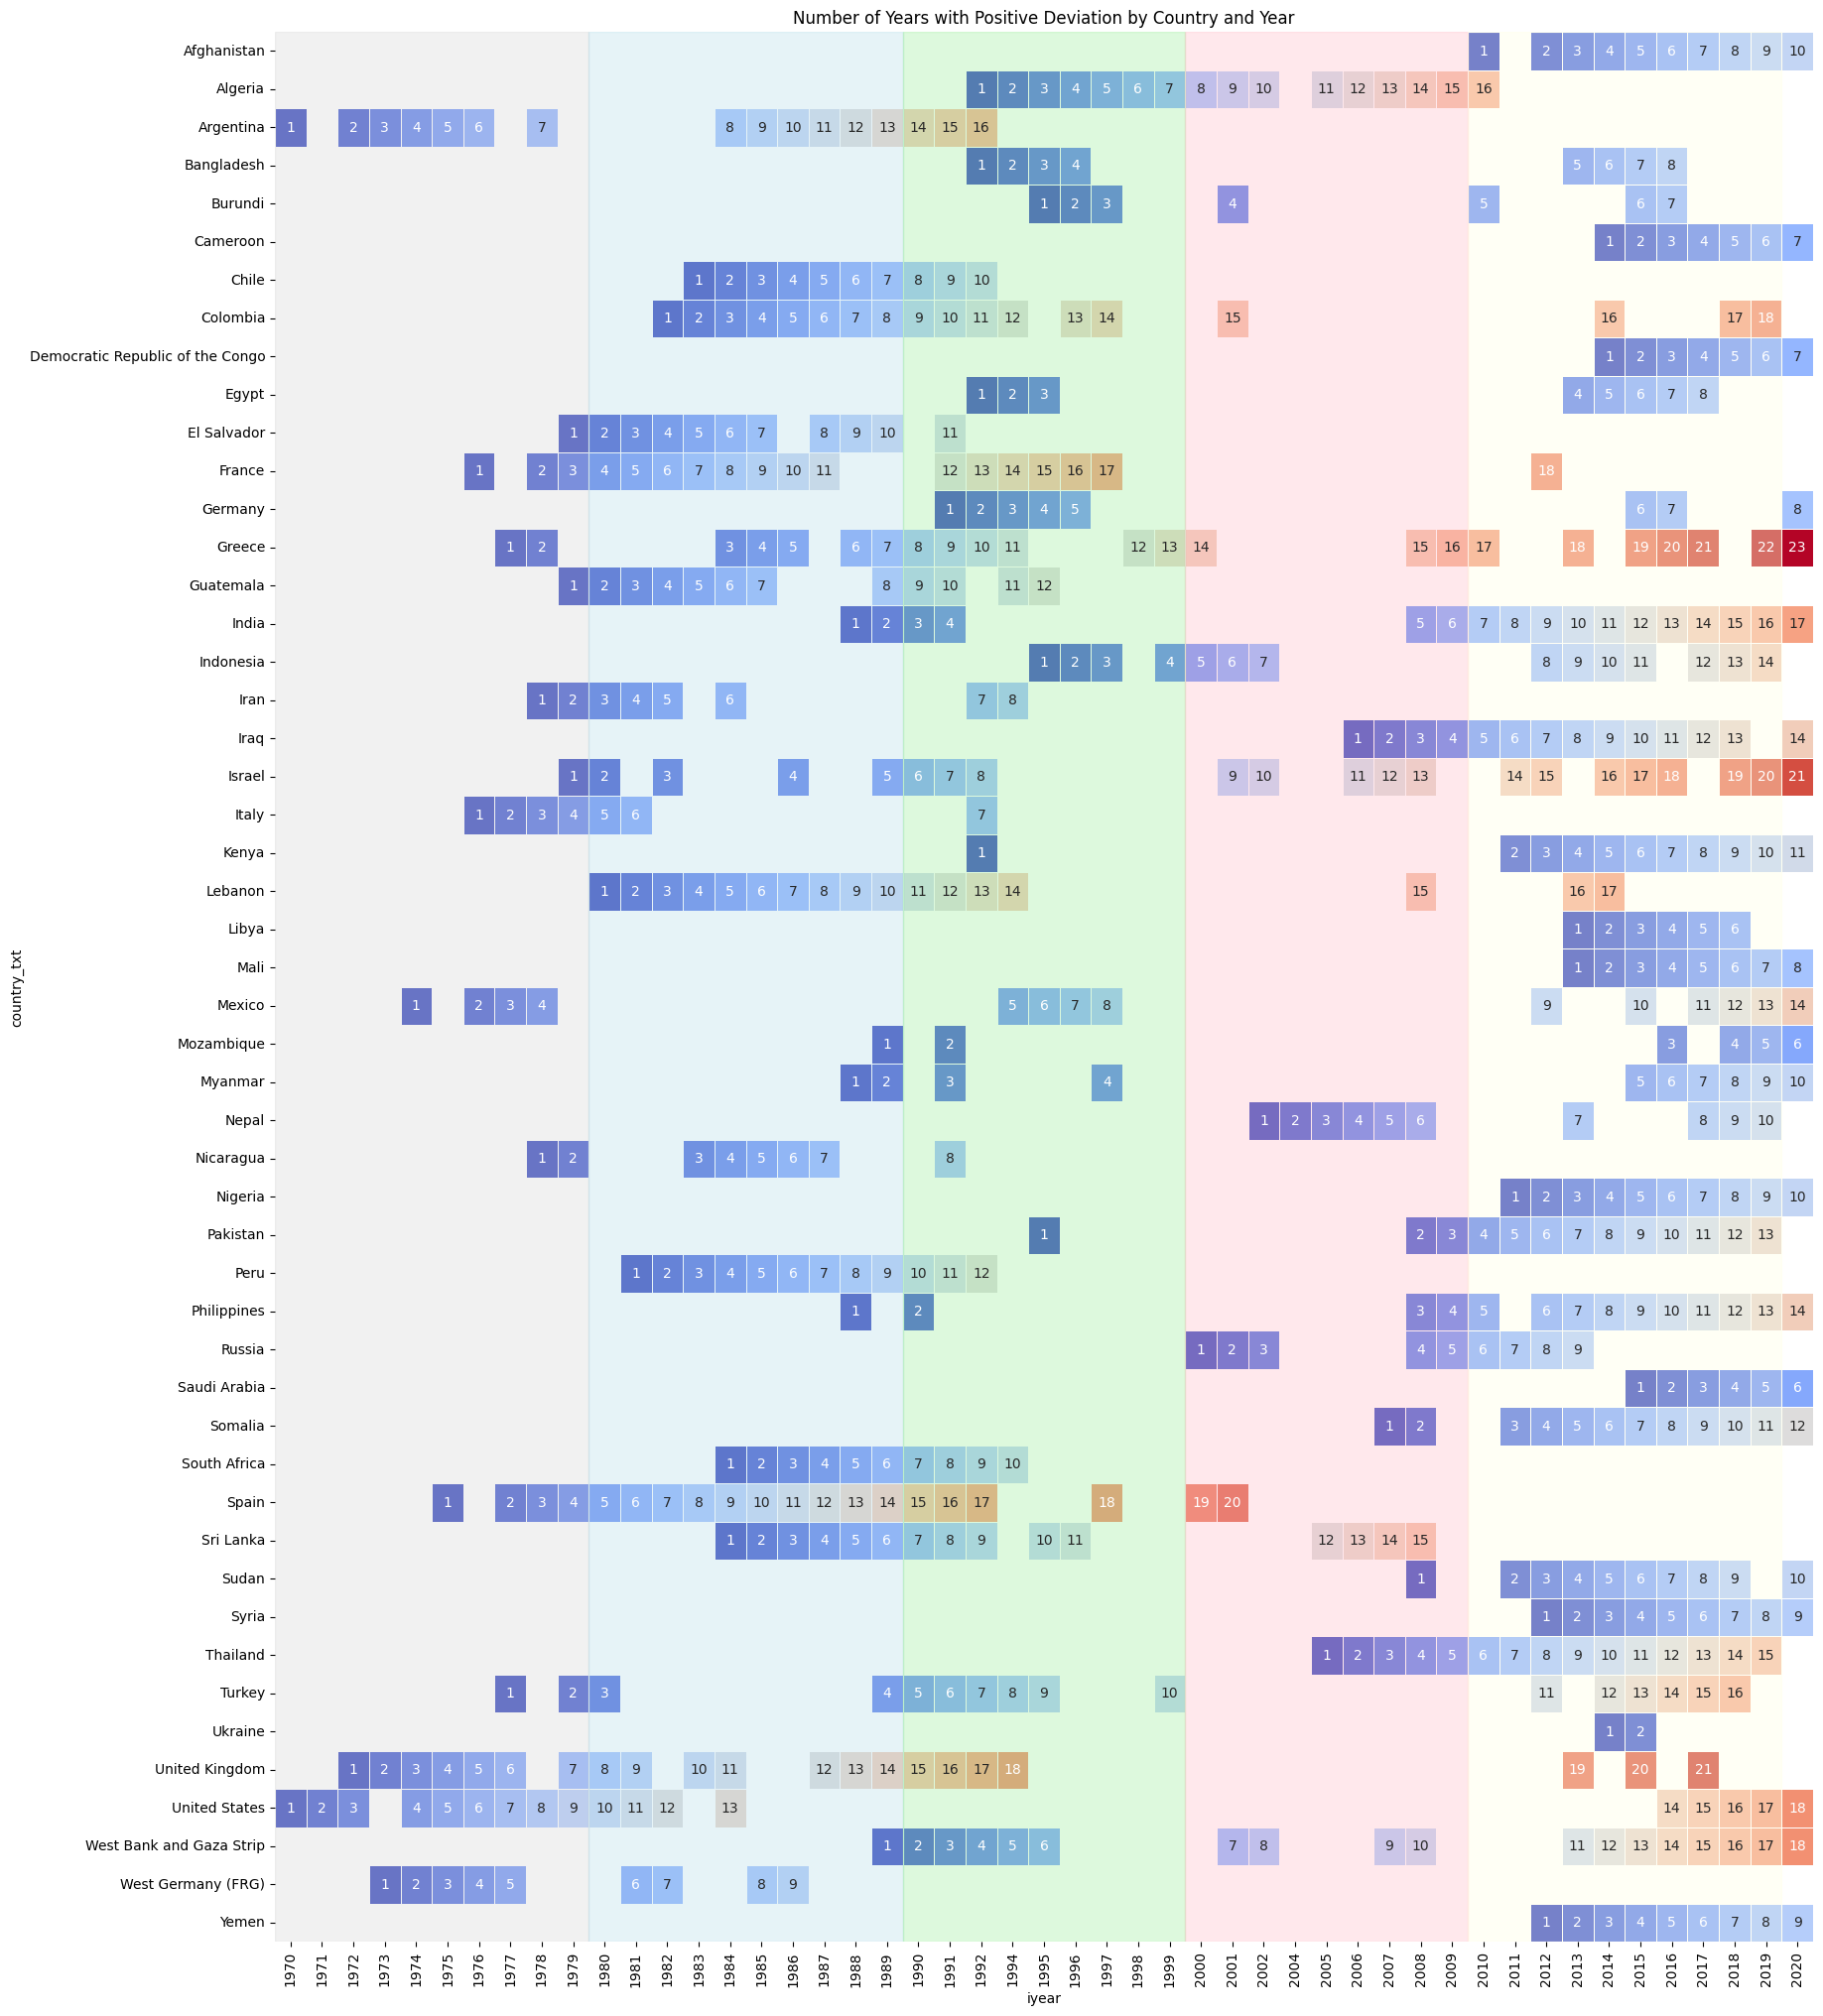
\includegraphics[width=0.5\linewidth]{img/Anomaly/anomaly_detect_heatmap_50_country.png}
    \caption{Heatmap Anomaly Detection}
    \label{fig:anomaly_detect_heatmap}
\end{figure}

\begin{figure}
    \centering
    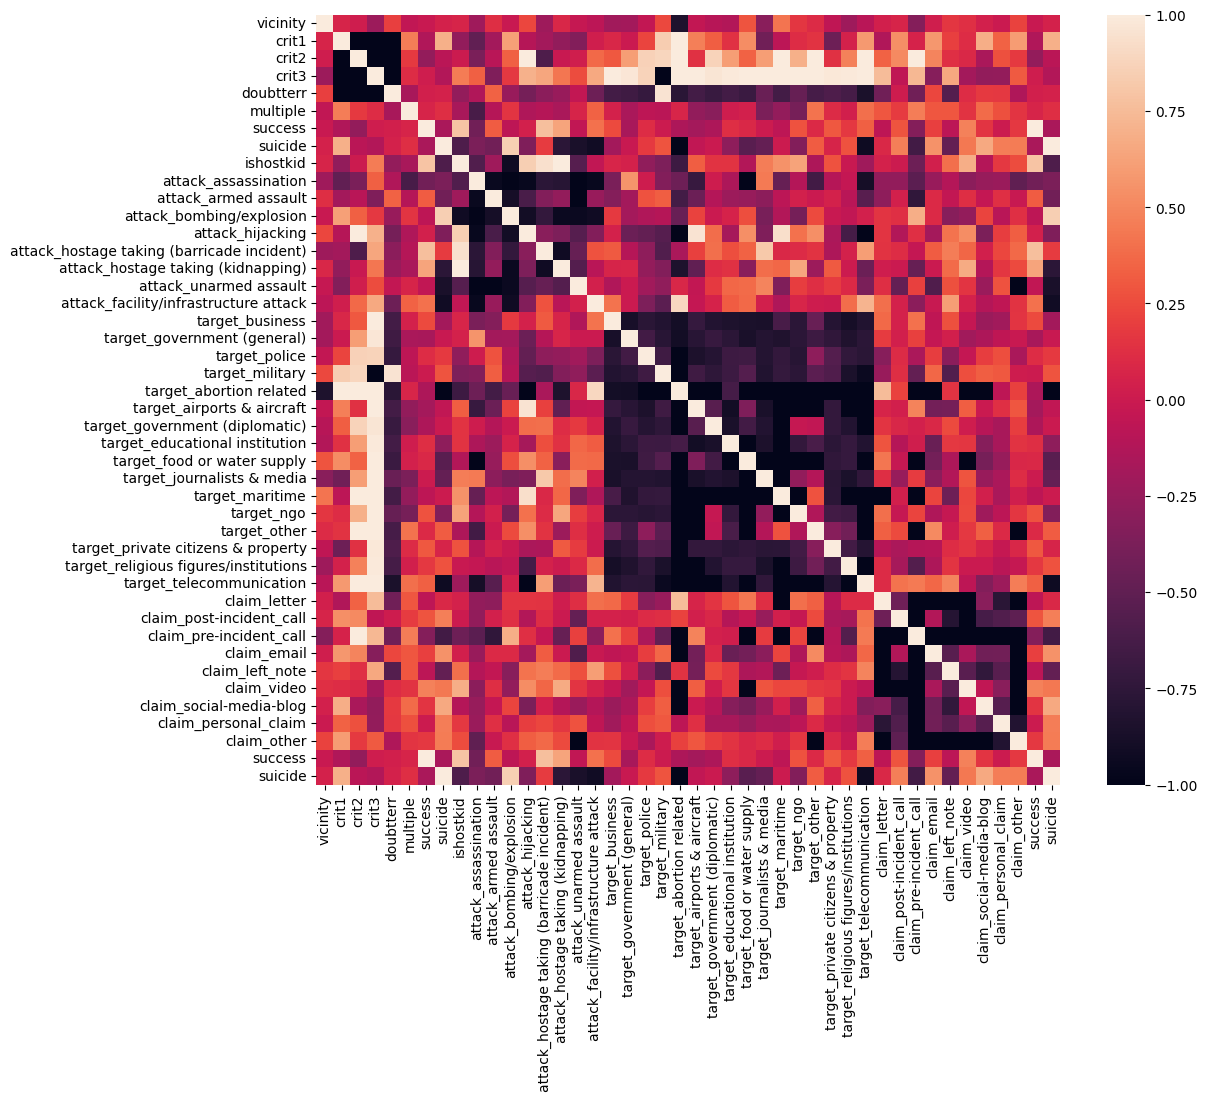
\includegraphics[width=1\linewidth]{img//Variable correlation/correlation_heatmap_2.png}
    \caption{Tetracoric correlation heatmap}
    \label{fig:tetracoric_heatmap}
\end{figure}

\begin{figure}
    \centering
    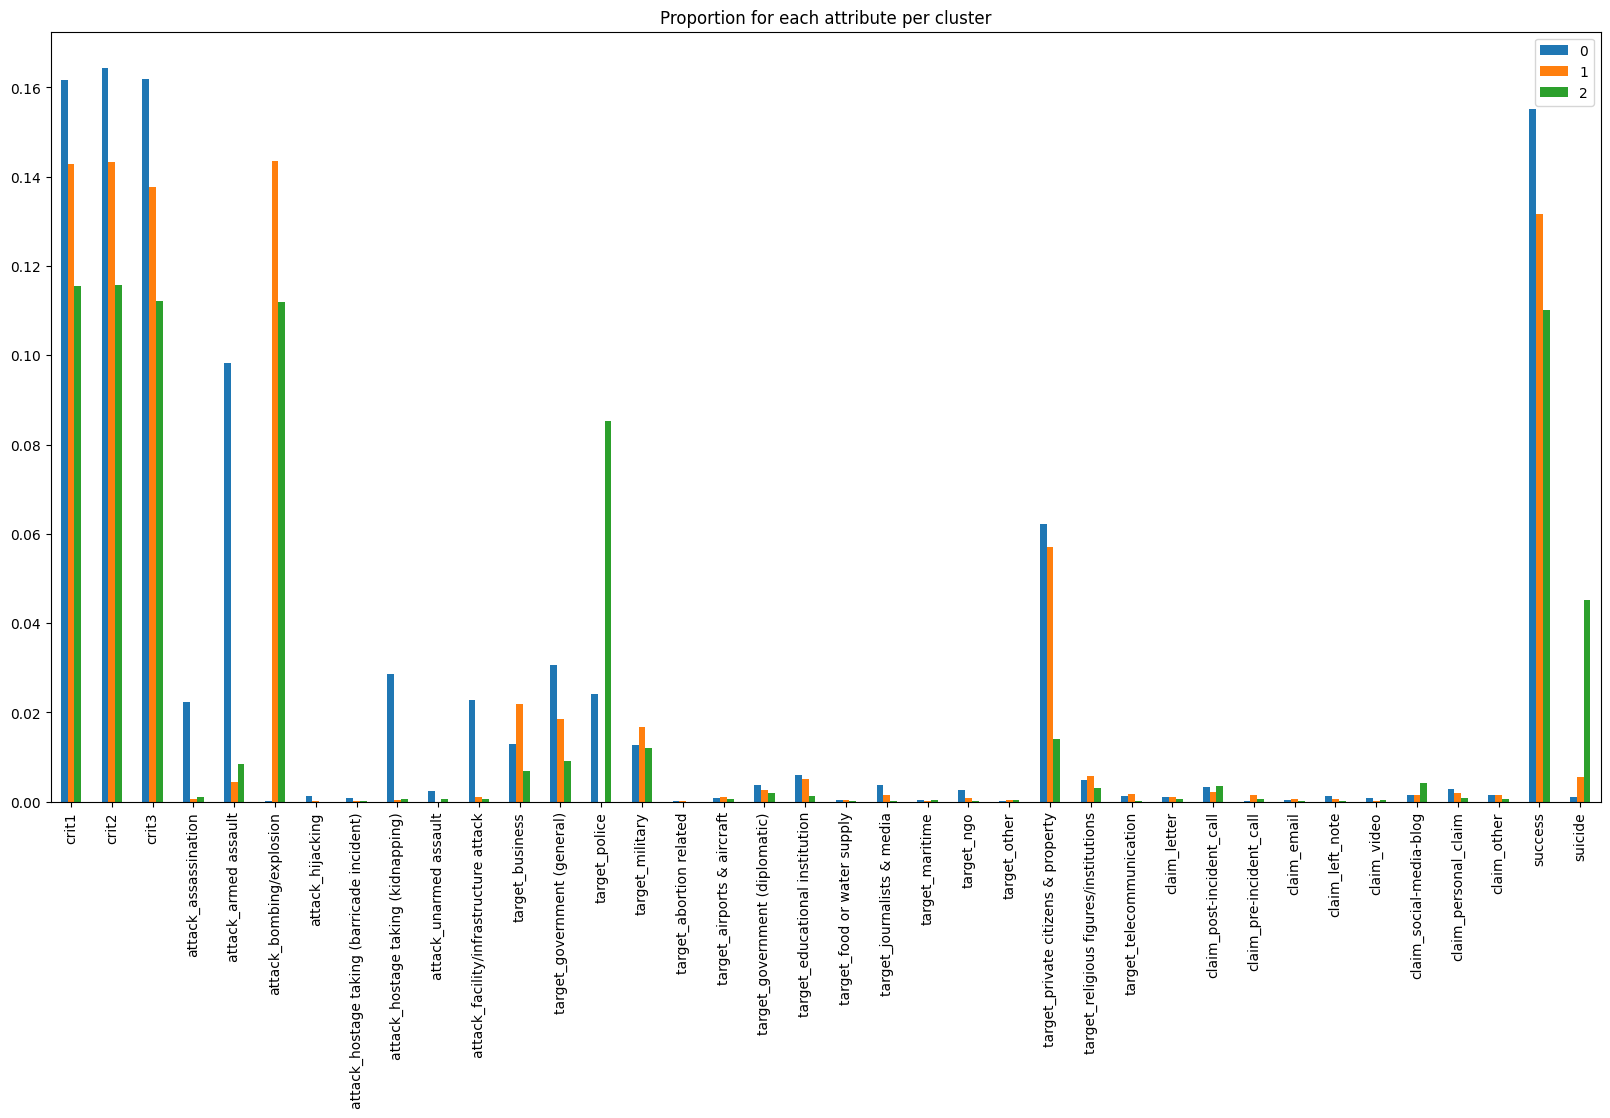
\includegraphics[width=0.90\linewidth]{img//Clustering/kmeans cluster propotions.png}
    \caption{Attribute proportion per cluster for the K-Means algorithm}
    \label{fig:kmeans-attributes}
\end{figure}

\begin{figure}
    \centering
    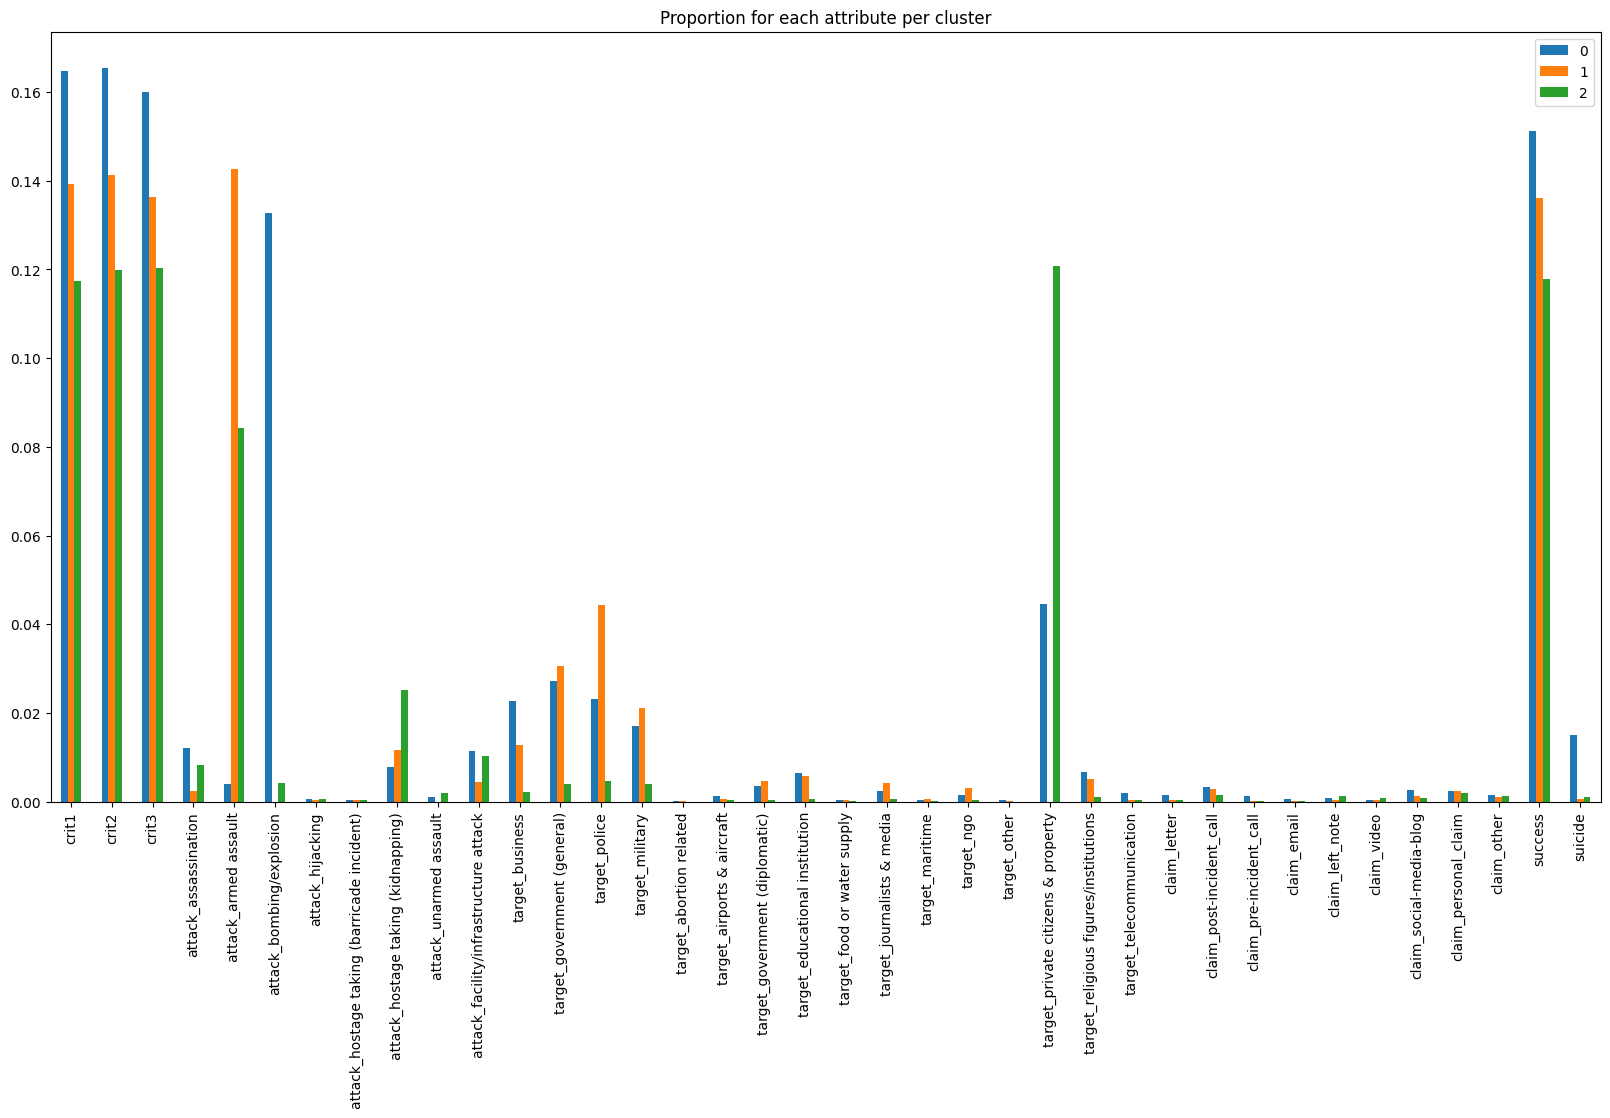
\includegraphics[width=0.90\linewidth]{img//Clustering/kmodes cluster propotions.png}
    \caption{Attribute proportion per cluster for the K-Modes algorithm}
    \label{fig:kmodes-attributes}
\end{figure}

\begin{figure}
    \centering
    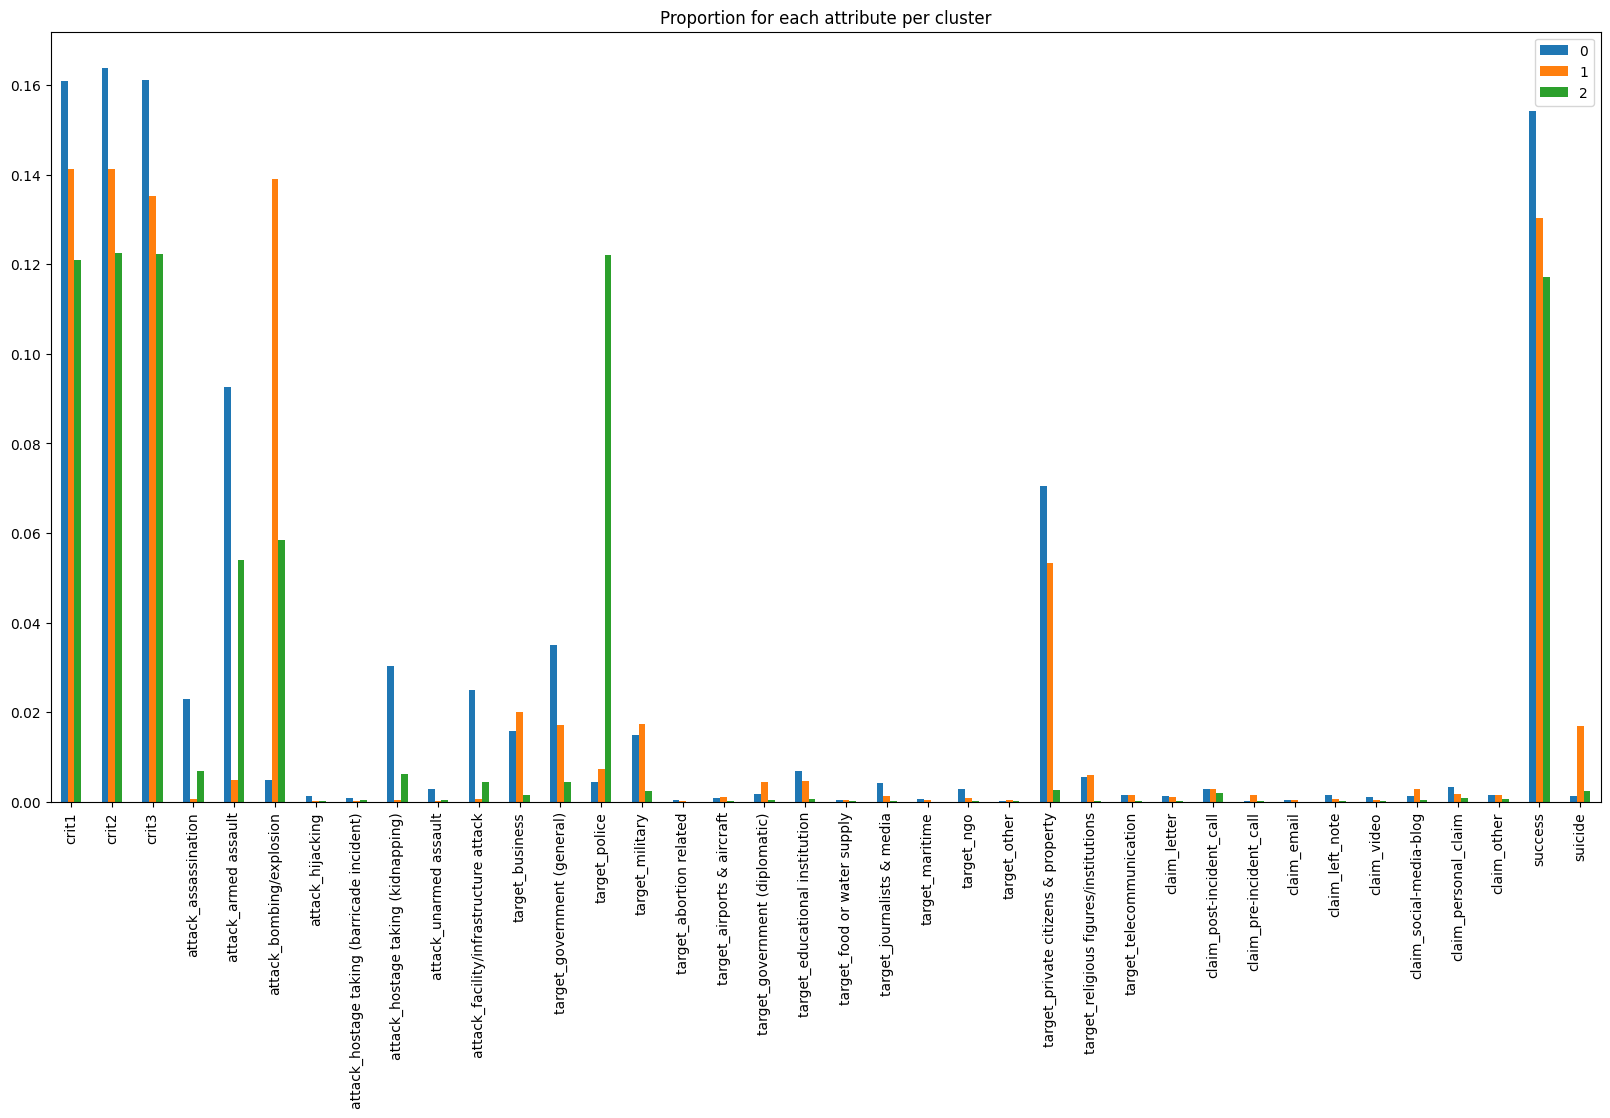
\includegraphics[width=0.90\linewidth]{img//Clustering/agglo cluster propotions.png}
    \caption{Attribute proportion per cluster for the Agglomerative clustering algorithm}
    \label{fig:agglo-attributes}
\end{figure}

\newpage
%\break
\printbibliography

\end{document}
    